\documentclass[11pt, letterpaper]{article}
\usepackage{geometry}
\usepackage[utf8]{inputenc}
\usepackage[tbtags]{amsmath}
\usepackage{amssymb}
\usepackage{gensymb}
\usepackage{physics}
\usepackage[makeroom,Smaller]{cancel}
\usepackage[dvipsnames]{xcolor}
\usepackage{tikz}

\usepackage{graphicx}
\graphicspath{ {./images/} }
\usepackage{subcaption}

% tikzplotlib
\usepackage{pgfplots}
%\DeclareUnicodeCharacter{2212}{−}
\usepgfplotslibrary{groupplots,dateplot}
\usetikzlibrary{patterns,shapes.arrows}
\pgfplotsset{compat=newest}

% footnote
\renewcommand{\thefootnote}{\fnsymbol{footnote}}

% Operators
\DeclareMathOperator*{\argmax}{arg\,max}
\DeclareMathOperator*{\argmin}{arg\,min}
\DeclareMathOperator*{\diag}{diag}
\newcommand{\exptval}[1]{\mathbb{E}\left[ #1 \right]}
\newcommand{\Var}[1]{\text{Var}\qty[#1]}
\newcommand{\Cov}[1]{\text{Cov}\qty[#1]}

% variables
\newcommand{\bb}[1]{\mathbb{#1}}
\newcommand{\vbd}{\vb{d}}
\newcommand{\vbm}{\vb{m}}
\newcommand{\vbep}{\vb{\varepsilon}}
\newcommand{\vbn}{\vb{n}}
\newcommand{\vbb}{\vb{b}}
\newcommand{\inv}[1]{#1^{-1}}
\newcommand{\noisevar}{\Sigma_{\vbn}}
\newcommand{\hatm}{\vb{\hat{m}}}
\newcommand{\Pdagger}{P^{\dagger}}
\newcommand{\Nbar}{\bar{N}}
\newcommand{\PPinv}[1]{\inv{\qty(\Pdagger #1 P)}}
\newcommand{\Neta}{N_{\eta}}


\title{Bai-Qiang Qiang Prospectus}
\author{Bai-Qiang Qiang}
\date{\today}

\begin{document}
\maketitle

\section{Introduction}
Cosmic microwave background is an electromagnetic radiation coming from early
stage of our universe. Based on hot Big Bang model, before the recombination
epoch, the photons were tightly coupled with free electrons and protons via 
Thomson scattering. As universe expanding and cooling down, free electrons and
protons combined into neutral hydrogen atom, this process is called 
recombination in cosmology. Shortly after this epoch, the photon could
propagate freely would not be scattered by charged particle. Now we received 
those photon produced at that time and called it cosmic microwave background
radiation. Studying these photons coming from early universe could help us
constrain theoretical model and cosmological constants
\cite{10.1093/ptep/ptaa104}.
The next generation CMB observations will have much higher resolution and 
genertes more data.
So we need an efficient way to processing data.
One of the these processing is map making, which gives an estimated map based 
on observation data.

Recently Elsner and Wandelt\cite{2013A&A...549A.111E} introduced a new
method called messenger field to solve Wiener filer, and then this technique
was being applied to map making equation\cite{Huffenberger_2018}.
It's been shown that this messenger field method is euquivalent to appling a
preconditioner to orignial problem and introduced an extra cooling parameter
$\lambda$, but whether this cooling parameter will boost performance compare to
conjugate gradient method is still controversial\cite{2018A&A...620A..59P}.
Here I'm gonna give a detailed analysis regarding this parameter and show that
it may improve proferformance under some circumstances, if we properly choose
its values.

The map making procedure could be summerized in equation
\begin{equation}
\vbd = P\vbm + \vbn \label{map making model}
\end{equation}
where $\vbd$, $P$, $\vbm$, $\vbn$ are time ordered data (TOD), pointing matrix,
CMB map, and noise.
The time ordered data we collected is given by map signal $P\vbm$ plus noise 
$\vbn$.
Pointing matrix $P$ acting on the map gives the signal of map at some specific 
position of sky where telescope is pointing at.
Here we could assume that the noise has zero mean $\ev{\vbn} = \vb{0}$,
since if it's not zero, we can always substract its mean value to make it zero.
And noise covariance matrix could be written as $N = \ev{\vbn \vbn^{\dagger}}$.

\section{Map Making Setup}
As we can see the map making model Eq.(\ref{map making model}) mathematically 
is a standard linear regression problem,
with \textit{design matrix} being pointing matrix $P$, and \textit{regression
coefficients} are $\vbm$.
Naturelly, we want to estimate linear regression coefficients $\vbm$,
with \textit{generalized least square} (GLS) technique.
The noise $\vbn$ is \textit{heteroscedastic}, its variance $N$ are 
different for various frequencies, usually detectors have $1/f$ noise pattern
\cite{1997PhRvD..56.4514T}.
The \textit{generalized least square} (GLS) will provide better estimation 
than \textit{ordinary least square} (OLS) method, because the data is
heteroscedastic so we would like to focusing on fitting the data with lower 
noise.

The GLS estimated map $\hatm$ is given by
\begin{equation}
\hatm = \argmin_{\vbm} (\vbd - P\vbm)^{\dagger} N^{-1} (\vbd - P \vbm) 
\label{GLS estimator equation}
\end{equation}
and we could define 
\begin{align}
\chi^2(\vbm) & \equiv (\vbd - P\vbm)^{\dagger} N^{-1} (\vbd - P \vbm) 
\label{chi2 formula}
\end{align}
therefore the estimated map $\hatm$ is the one minimize $\chi^2(\vbm)$.
To find out expression for $\hatm$, we first take derivative with respect to 
vector $\vbm$
\begin{align}
\begin{aligned}[b]
\pdv{\vbm} \chi^2(\vbm)
&= \pdv{\vbm} (\vbd - P\vbm)^{\dagger} N^{-1} (\vbd - P \vbm)
\\
&= \pdv{\vbm} \qty\Big(
    \vbd^{\dagger} N^{-1} \vbd 
    - \vbd^{\dagger} N^{-1} P \vbm 
    - \vbm^{\dagger}\Pdagger N^{-1}\vbd 
    + \vbm^{\dagger} \Pdagger N^{-1}P\vbm
)
\\
&= -2\Pdagger N^{-1} \vbd + 2 \Pdagger N^{-1} P \vbm
\label{dchi2/dm}
\end{aligned}
\end{align}
then set it equals to zero $\pdv{\vbm} \chi^2(\hatm) = 0$,
we get the \textit{map making equation}
\begin{align}
\hatm = \PPinv{N} \Pdagger \inv{N} \vbd \label{map making equation}
\end{align}
This is also called COBE method for map making.

\section{Some Nice Proporties}

\subsection{Unbiased linear estimator}
Linear estimator means $\hatm$ could be written as $\hatm = W\vbd$,
it's linear combination of $\vbd$.
We say the estimator is unbaised if
\begin{align}
\begin{aligned}[b]
&\mathrel{\phantom{\Rightarrow}}\ev{\hatm} = m \\
&\Rightarrow\ev{W \vbd} = m\\
&\Rightarrow\ev{W(Pm + \vbn) } = m \\
&\Rightarrow WP = I
\end{aligned}
\end{align}
At last step we used the property  $\ev{\vbn} = 0$.
And for the generalized least square estimator matrix 
$W = \PPinv{N} \Pdagger \inv{N}  $, which satisfy the condition $WP=I$.
Therefore $\hatm$ is unbaised estimated map.


\subsection{Minimize variance $\Var{\hatm_i}$ under constrain of unbaised 
linear estimators} \label{minimize variance}
The covariance of the estimator $\hatm = W \vbd$ is
\begin{align}
\begin{aligned}[b]
\Cov{\hatm} &= \Cov{W\vbd} 
\\ 
&= \Cov{WP\vbm + W\vbn} 
\\ 
&= \Cov{W\vbn} 
\\ 
&= W N W^{\dagger} \label{covariance hatm}
\end{aligned}
\end{align}

Here we use a trick \cite{weighted_and_GLS},
if consider the matrix $W = W_{GLS} + W'$ where
$W_{GLS} = \PPinv{N} \Pdagger \inv{N} $ is the matrix for GLS estimation,
and in order to satisfy the condition $WP = I$, we should have $W'P = 0$.
Then the covariance matrix
\begin{align}
\begin{aligned}[b]
\Cov{\hatm }
&= W_{GLS} N W_{GLS}^{\dagger} + W' N W'^{\dagger} 
    + W_{GLS} N W'^{\dagger} + W' N W_{GLS}^{\dagger}
\\
&= \PPinv{N} + W' N W'^{\dagger} 
    + \PPinv{N} \Pdagger W'^{\dagger} + W' P \PPinv{N}
\\
&= \PPinv{N} + W' N W'^{\dagger} 
\end{aligned}
\end{align}
where the last line used condition $W'  P = 0$.

The variance $\Var{\hatm_i}$ is diagonal elements of covariance matrix
$\Cov{\hatm}$
\begin{align}
\begin{aligned}[b]
\Var{\hatm_i}
&= \qty\Big{ \PPinv{N}}_{ii} + \qty\big{W' N W'^{\dagger}}_{ii}
\\
&= \qty\Big{ \PPinv{N}}_{ii} + W'_{i,:} N W'^{\dagger}_{i,:}
\end{aligned}
\end{align}
where $W'_{i,:}$ is the $i^{th}$ row vector of $W'$.
Since the noise covariance matrix $N$ is positive semidefinite matrix,
therefore $W'_{i,:} N W'^{\dagger}_{i,:} \geq 0$.
If $W' = 0$ Then we have $W = W_{GLS}$, variance $\Var{\hatm_i}$ would have 
its minimum variance. 

\subsection{Minimize mean square error under constrain of unbaised linear 
estimator}
The error is defined as the difference between estimated map and real one
\begin{align}
\begin{aligned}[b]
\vbep &\equiv \hatm - \vbm
\\
&= W\vbd - \vbm
\\
&= (WP-I)\vbm + W\vbn
\\
&= W\vbn
\end{aligned}
\end{align}
where the last line used relation $WP=I$ for unbaised estimator $W$. 

Now we need to minimize mean square error
\begin{align}
\begin{aligned}[b]
\ev{\vbep^{\dagger} \vbep }
&= \ev{\Tr(\vbep \vbep^{\dagger})}
\\
&=\ev{\Tr(W\vbn \vbn^{\dagger} W^{\dagger}) }
\\
&= \Tr(W N W^{\dagger})
\\
&= \Tr(\Cov{\hatm})\\
&= \sum_i \Var{\hatm_i}
\end{aligned}
\end{align}
the second line we used property $\vbep^{\dagger} \vbep$ is a scalar,
so $\vbep^{\dagger} \vbep = \Tr(\vbep^{\dagger} \vbep) 
= \Tr(\vbep \vbep^{\dagger})$,
and the fourth line is because trace is a linear operation 
and $\ev{\vbn \vbn^{\dagger} } = N$, 
the fifth line comes from Eq.(\ref{covariance hatm}).
In Section \ref{minimize variance} we have shown that the generalized least 
square matrix $W_{GLS}$ minimize $\Var{\hatm_i}$ for each $i$, 
therefore it also minimize the mean square error
$\ev{\vbep^{\dagger} \vbep} = \sum_i \Var{\hatm_i}$. 

\subsection{Maximum likelihood estimator}
Previous proporties does not depends on the noise distribution, 
if we assume that the noise is multivariate normal distributed
$\vbn \sim \mathcal{N}(0, N)$ with mean $0$ covariance $N$.
Its likelihood function will be
\begin{align}
L\qty(\vbd;\vbm) = \frac{1}{\sqrt{(2\pi)^n \abs{N}}} 
    \exp(-\frac{1}{2} \qty(\vbd - P\vbm)^{\dagger} N \qty(\vbd - P\vbm))
\end{align}
and Log-likelihood
\begin{align}
\log\qty(L\qty(\vbd;\vbm))
= -\frac{1}{2} \qty(\vbd - P\vbm)^{\dagger} N \qty(\vbd - P\vbm) + \text{cont.}  
\end{align}
maximazing this log-likelihood function with respect to $\vbm$, is equivalent
to minimize $\chi^2(\vbm) =\qty(\vbd - P\vbm)^{\dagger} N \qty(\vbd - P\vbm)$,
which is $\hatm$.

\section{Solve Map Making Equation}

The map making equation Eq.(\ref{map making equation}) derived from Generalized
Least Square estimation,
\begin{align}
\qty(\Pdagger \inv{N}  P) \hatm = \Pdagger \inv{N} \vbd \label{map making eq}
\end{align}
If we define $A = \Pdagger \inv{N} P$ and $b = \Pdagger \inv{N} d$,
then it could be written as $A\hatm = \vbb$.

Based on current computation power, it is impossible to solve $\hatm$
by calculating $\hatm = \PPinv{\inv{N}} \Pdagger \inv{N} \vbd$ directly,
since the noise covariance matrix $N$ is sparse in frequency domain,
and pointing matrix $P$ is sparse in (time by pixel) domain.
It's impossible to do these matrix multiplication directly and then take
inverse.
However, for a vector with size of map $\hatm$, we could caculte
$\Pdagger \inv{N} P \hatm = A\hatm$ by first taking Fourier transform $P\hatm$
then inverse Fourier transform $\inv{N}P\hatm$.
Which means it could be solved by conjugate gradient method.


\subsection{Preconditioner}
To improve the preformance of conjugate gradient method,
we could apply preconditioner $M$ to original problem $A\hatm = \vbb$,
which then becomes $\inv{M}A\hatm = \inv{M} \vbb$.
The preconditioner should reduce condition number of original problem,
such that conjugate gradient method would converge faster.
We want the preconditioner to capture as much information as possible from 
matrix $A$, but still keep it relative easy to calculate $\inv{M}$.
For example, if $M = A$, $\inv{M} A \hatm = \inv{M} \vbb$ would be solved
immediatly, but $\inv{M}$ will be extremly difficulte to calculate.
We could simply choose $M = \Pdagger P$,
and the operation $\inv{M} \vbm = \PPinv{} \vbm$ is average over each pixel 
of map $\vbm$.

For conjugate gradient method, we need a initial guess map $\hatm_0$. 
Sure we can use zero vector $\hatm_0 = \vb{0}$ as initial guess,
but simple binned map $\hatm_0 = \PPinv{} \Pdagger \vbd$ would be a better 
choice, which is a the solution for white noise case $N \propto I$.
(Pape\v{z} et al. 2018\cite{2018A&A...620A..59P}) showed that using 
$\hatm_0$ as initial guess could imporove performace significantly compare to
zero vector $\vb{0}$ in come cases.
As stated before we can calculate $\PPinv{}$ acting on any map size object,
and $\Pdagger \vbd$ is indeed a map size object, 
so we could obtain simple binned map by calculating
$\hatm_0 = \PPinv{} \Pdagger \vbd$ directly.

For conjugate gradient method with simple preconditioner $M = \Pdagger P$,
we've got all we need.
Next we only need to use conjugate gradient algorithm solve the problem.

\subsection{Parameterized Conjugate Gradient Method}

We could also parameterize map making equation Eq.(\ref{map making eq}),
and it may improve performace in some cases.
The idea is that map making equation Eq.(\ref{map making eq}) is hard to solve
due to noise covariance matrix is sandwitched between $\Pdagger P$.
But if noise covariance matrix $N$ is proportional to identity matrix $I$, 
then its solution is given by simple binned map
$\vbm_0 = \inv{\qty(\Pdagger P)} \Pdagger \vbd$,
which could be solved directly. 
So what if we parameterize noise covariance matrix $N$ with a parameter $\eta$,
such that initally $\eta = \eta_i$, $N\qty(\eta_i) \propto I$ 
and final $\eta = \eta_f$ and $N\qty(\eta_f) \propto N$,
such that the final solution is what we want.
We expect the parameterized noise covariance matrix $N(\eta)$
would connect our inital guess $\hatm_0$ and final solution $\hatm$ as we 
change $\eta$ from $\eta_i$ to $\eta_f$.

Now instead of Eq.(\ref{map making eq}), we are solving
\begin{align}
\qty(\Pdagger \inv{N(\eta)} P)\, \hatm(\eta) 
= \Pdagger \inv{N(\eta)} \vbd \label{map making para}
\end{align}

Now question is how to find $N(\eta)$ such that $N(\eta_i) \propto I$
and $N (\eta_f) \propto N$?
Since the non white noise part of $N$ is a trouble maker,
we could think of it as a perturbative term, which add upon the white noise.
Initially there is only white noise and solution is given by $\hatm_0$,
then we gradually add extra noise into this equation by changing $\eta$ from 
$0$ to $1$.
At the end when $\eta=1$ we are solving equation Eq.(\ref{map making eq}).

Therefore we separate noise covariance matrix into two parts
$N = \tau I + \Nbar$ where $\tau$ is the minimum eigenvalue of $N$. 
Then we define $N(\eta) = \tau I + \eta \Nbar$, 
with perturbative parameter $\eta$ which satisfies $\eta_i = 0$ and $\eta_f=1$.

Eq.(\ref{map making para}) then becomes
\begin{align}
\qty(\Pdagger \inv{(\tau I + \eta \Nbar)}P) \, \hatm(\eta) 
= \Pdagger \inv{\qty(\tau I + \eta \Nbar)} \vbd \label{map making perturb} 
\end{align}

We require the perturbative parameter $\eta$ being monotonically increase
series $0 = \eta_0 < \eta_1 < \cdots < \eta_n = 1$.
For some specific $\eta_m$, we use conjugate gradient method to solve equation 
$\qty(\Pdagger \inv{N(\eta_m)} P)\, 
\hatm(\eta_m) = \Pdagger \inv{N(\eta_m)} \vbd$
with simple preconditioner $\Pdagger P$,
and using $\hatm(\eta_{m-1})$ as the inital value.
The initial guess $\hatm(\eta_0) = \vbm_0 = \PPinv{} \Pdagger \vbd$.


\subsubsection{Choosing perturbative parameters $\eta$}
Next question is how we choose these monotonically increasing parameters
$\eta$. 
If we choose these parameters inappropriately, it would only makes it converge
slower.
Also we want to determin $\eta_1, \cdots, \eta_{n-1}$ before starting conjugate
gradient iteration.
That's because time ordered data $\vbd$ is very large,
and we don't want to keep it at system RAM during calculation.
If $\eta_1, \cdots, \eta_{n-1}$ could be determined before the iterations, 
then we can first calculate $\Pdagger \inv{N(\eta)} \vbd$ for each $\eta_m$
and store these map sized object in RAM,
instead of entire time ordered data $\vbd$.

First let's try to find out our starting point $\eta_1$.
What would be good value for $\eta_1$?

Here to simplify notation, I will use $\Neta$ denote $N(\eta)$.
The estimated map
$\hatm(\eta) = \PPinv{\inv{\Neta}} \Pdagger \inv{\Neta} \vbd$
minimize
\begin{align}
\chi^2 (\vbm, \eta)
= \qty(\vbd - P \vbm)^{\dagger} \inv{\Neta} (\vbd - P\vbm)
\label{chi2 eta formula}
\end{align}
For some specific $\eta$ value, the minimum $\chi^2$ value is given by
\begin{align}
\begin{aligned}[b]
\chi^2 (\hatm(\eta), \eta)
&= \qty\big(\vbd - P \hatm(\eta))^{\dagger} \inv{\Neta} 
    \qty\big(\vbd - P\hatm(\eta))
\\
& = \vbd^{\dagger} \qty[\inv{\Neta}
    - \inv{\Neta}P\inv{\qty[
        \Pdagger \inv{\Neta} P
    ]}\Pdagger\inv{\Neta}]\vbd
\end{aligned}
\end{align}
Now let's see how $\chi^2(\hatm(\eta),\eta)$ changes as we change $\eta$.
\begin{align}
\begin{aligned}[b]
\dv{\eta} \chi^2(\hatm(\eta),\eta) 
&= \dv{\eta}(\vbd^{\dagger}\inv{\Neta}\vbd)
    - \dv{\eta}(
        \vbd^{\dagger}\inv{\Neta}P 
        \PPinv{\Neta} 
        \Pdagger \inv{\Neta} \vbd
    )
\\
&= \vbd^{\dagger} \inv{\Neta} \bigl[
    - \Nbar
    + \Nbar \inv{\Neta}P\PPinv{\Neta}\Pdagger
    \\
    &\phantom{= \vbd^{\dagger} \inv{\Neta} \bigl[}
    -P\PPinv{\inv{\Neta}} \Pdagger \inv{\Neta} \Nbar \inv{\Neta}
        P \PPinv{\inv{\Neta}}\Pdagger
    \\
    &\phantom{= \vbd^{\dagger} \inv{N_{\eta}} \bigl[}
    + P \PPinv{\inv{\Neta}} \Pdagger \inv{\Neta} \Nbar
    \big] \inv{\Neta} \vbd
\end{aligned}
\end{align}
Simplify this expression with identity
$\hatm = \PPinv{\inv{\Neta}} \Pdagger \inv{\Neta}\vbd$, and yields
\begin{align}
\dv{\eta} \chi^2(\hatm(\eta), \eta) 
&= - \qty(\vbd - P\hatm(\eta))^{\dagger} \inv{\Neta} \Nbar \inv{\Neta} 
    (\vbd - P\hatm(\eta)) \label{d chi2}
\end{align}
also notice that
$\dv{\eta} \chi^2(\hatm(\eta), \eta) = \pdv{\eta} \chi^2(\hatm(\eta), \eta)$,
because by the definition of $\hatm(\eta)$ it minimize
$\chi^2(\vbm, \eta)$ for some fixed $\eta$ value,
implies $\pdv{\vbm} \chi^2(\hatm(\eta), \eta) = 0$.


To further simplify analysis, let's assume that the noise covariance matrix
$N = \ev{\vbn\vbn^{\dagger}}$ is diagnal under frequency domain.
Therefore $\Nbar$ and $\Neta$ are also diagnal in frequency domain by
definition, and all the diagnal elements are greater than or equal to zero,
because covariance matrix is positive semi-definite.
Also, we can conclude that matrix
$\inv{\Neta} \Nbar \inv{\Neta}$ is positive semi-definite matrix.
Based on Eq.(\ref{d chi2}), we know that
$\dv{\eta} \chi^2({\hatm(\eta), \eta}) \leq 0$,
so $\chi^2(\hatm(\eta), \eta)$ is always decrease
as $\eta$ changes from $0$ to $1$.

The relative decrease of $\chi^2(\hatm(\eta), \eta)$ at $\eta$ is defined as
\begin{align}
\begin{aligned}[b]
-\frac{\delta \chi^2(\hatm(\eta),\eta)} {\chi^2(\hatm(\eta), \eta)}
&=
-\delta \eta \frac{1}{\chi^2(\hatm(\eta), \eta)} \, 
\dv{\eta} \chi^2(\hatm(\eta), \eta) 
\\&= 
\delta \eta 
\frac{\qty(\vbd - P\hatm(\eta))^{\dagger}
    \inv{\Neta} \Nbar \inv{\Neta}
    (\vbd - P\hatm(\eta)) 
}
{\qty\big(\vbd - P \hatm(\eta))^{\dagger} 
    \inv{\Neta}
    \qty\big(\vbd - P\hatm(\eta))
}
\end{aligned}
\end{align}
Here we put a minus sign in front of
$\delta\chi^2(\hatm(\eta), \eta)/\chi^2(\hatm(\eta), \eta)$,
such that it's non-negative.
If we choose $\eta_1 = \eta_0 + \delta\eta = \delta\eta$
such that $\eta_1 = \delta \eta$ is very small quantity.
Then the relative decrease from $\eta_0= 0$ to $\eta_1 = \delta \eta$ is
\begin{align}
\begin{aligned}[b]
-\frac{\delta \chi^2(\hatm(0), 0)}{\chi^2(\hatm(0), 0)} 
&= \delta \eta 
\frac{1}{\tau}
\frac{\qty(\vbd - P\hatm(0))^{\dagger} \Nbar  (\vbd - P\hatm(0)) }
    {\qty\big(\vbd - P \hatm(0))^{\dagger} \qty\big(\vbd - P\hatm(0))}
\\
& \leq  \frac{\delta \eta}{\tau} \max(\Nbar_f)
\end{aligned}
\end{align}
where at first line we used the property $N_{\eta=0} = \tau I$,
and second line because positive semi-definite $\Nbar$ is diagnal in frequency 
domain its maximum eigenvalue is $\max(\Nbar_f)$.
To prove this, notice that matrix $\Nbar$ is diagnalized in frequency space 
with eigenvalues $\Nbar_f\geq0$ and corresponding eigenvector $\vb{e}_f$
(these eigenvectors form a complete orthonornal basis),
any vector could be decomposed into these frequency basis
$\vb{v} = \sum_f \alpha_f \vb{e}_f$, therefore we have
$\frac{\vb{v}^{\dagger} \Nbar \vb{v}}{\vb{v}^{\dagger} \vb{v}} 
= \frac{\sum_f \alpha_f^2\Nbar_f}{\sum_f \alpha_f^2}
\leq \max(\Nbar_f) $

Ideally, we want
$\delta \chi^2(\hatm(0),0) = \chi^2(\hatm(1), 1) - \chi^2(\hatm(0),0)$,
such that it would get close to final $\chi^2$ at next iteration.
Here if we assume that initial $\chi^2$ value $\chi^2(\hatm(0),0)$ is much
larger than final value $\chi^2(\hatm(1),1)$,
then we would expect
$\qty|\delta\chi^2(\hatm(0),0)/\chi^2(\hatm(0),0)| \approx 1^-$.
To make sure it won't going too fast, we don't want 
$\qty|\delta\chi^2(\hatm(0),0)/\chi^2(\hatm(0),0)|$ 
exceeds $1$.
So we could set upper bound $\delta \eta \max(\Nbar_f) / \tau = 1$
and set
\begin{equation}
\eta_1 = \frac{\tau}{\max(\Nbar_f)} = \frac{\min(N_f)}{\max(N_f) - \min(N_f)}
\end{equation}
Here $N_f$ is the eigenvalues of noise covariance matrix $N$ under frequency
domain.
If the condition number of noise covariance matrix
$\kappa(N) = \max(N_f)/\min(N_f) \gg 1$,
then $\eta_1 \approx \inv{\kappa} (N)$.

What about other parameters $\eta_m$ with $m > 1$?
We could use similar analysis,
suppose $\eta_{m+1} = \eta_m + \delta \eta_m$ with small $\delta\eta_m$,
and the relative decrese
\begin{align}
\begin{aligned}[b]
-\frac{\delta \chi^2(\hatm(\eta_m), \eta_m)}{\chi^2(\hatm(\eta_m), \eta_m)}  
&= \delta\eta_m
\frac{\qty(\vbd - P\hatm(\eta_m))^{\dagger}
    \inv{N_{\eta_m}} \Nbar \inv{N_{\eta_m}}
    (\vbd - P\hatm(\eta_m))
}
{\qty\big(\vbd - P \hatm(\eta_m))^{\dagger}
    \inv{N_{\eta_m}}
    \qty\big(\vbd - P\hatm(\eta_m))
}
\\
& \leq \delta \eta_m\, \max\qty(\frac{\Nbar_f}{\tau + \eta_m \Nbar_f})
\label{eta upper bound}
\end{aligned}
\end{align}
The upper bound at second line is a little bit tricky.
Both matrix $\Nbar$ and $\inv{N}_{\eta_m}$ 
can be simultaneously diagnalized in frequency space.
For each eigenvector $\vb{e}_f$
the corresponding eigenvalue of the matix 
$\inv{N}_{\eta_m} \Nbar \inv{N}_{\eta_m}$
is
$\lambda_f = \Nbar_f (\tau + \eta_m \Nbar_f)^{-2}$,
and the eigenvalue for matrix 
$\inv{N}_{\eta_m}$
is
$\gamma_f = (\tau + \eta_m \Nbar_f)^{-1}$.
Their eigenvalues are related by
$\lambda_f = \frac{\Nbar_f}{\tau + \eta_m \Nbar_f} \gamma_f$.
For any vector $\vb{v} = \sum_f \alpha_f \vb{e}_f$, we have
$\frac{\vb{v}^{\dagger} \inv{N}_{\eta_m} \Nbar \inv{N}_{\eta_m} \vb{v}}
{\vb{v}^{\dagger} \inv{N}_{\eta_m} \vb{v}}
= \frac{\sum_f \alpha_f^2 \lambda_f}{\sum_f \alpha_f^2 \gamma_f}
= \frac{\sum_f \alpha_f^2 \gamma_f \Nbar_f/(\tau + \eta_m \Nbar_f)}
{\sum_f \alpha_f^2 \gamma_f}
\leq \max \qty( \frac{\Nbar_f}{\tau + \eta_m \Nbar_f})
$

Similarly, we could set the upper bound
$\delta\eta_m \max \qty( \frac{\Nbar_f}{\tau + \eta_m \Nbar_f})=1$,
\footnote{Here we also assmumed that
$\chi^2(\hatm(\eta_m),\eta_m) \gg \chi^2(\hatm(1),1)$,
which we expect it to be satisfied for $0 \simeq \eta_m \ll 1$. 
Since final result Eq.(\ref{etai rule}) is geometric series,
only a few $\eta_m$ values won't satisfy this condition.
}
then we get
\begin{align}
\delta \eta_m 
= \min \qty(\frac{\tau + \eta_m \Nbar_f}{\Nbar_f})
= \eta_m + \frac{\tau }{\max(\Nbar_f)}
\end{align}
Therefore 
\begin{align}
\eta_{m+1} = \eta_m + \delta\eta_m = 2\eta_m + \frac{\tau }{\max (\Nbar_f)}
\end{align}
As we can see, $\eta_1, \cdots, \eta_n$ should increase like a geometric
series. 
And written in the form $\eta_{m+1} + \frac{\tau }{\max(\Nbar_f)}
= 2 \qty( \eta_m + \frac{\tau}{\max(\Nbar_f)})$
it's easy to see that for $m \geq 1$,
$\eta_{m} + \frac{\tau }{\max(\Nbar_f)}$ forms a geometric series
\begin{align}
\eta_m +  \frac{\tau }{\max(\Nbar_f)}
=\qty(\eta_1 + \frac{\tau }{\max(\Nbar_f)}) 2^{m-1}
=\frac{\tau}{\max(\Nbar_f)} 2^m
\end{align}
Note that $m = 0$ and $\eta_0 = 0$ also satisfy this expression and we've got
final expression for all $\eta_i$
\begin{align}
\eta_i =\min \qty\bigg{1,\; \frac{\tau}{\max(\Nbar_f)} \qty(2^i -1) }
\label{etai rule}
\end{align}
Here we need to truncate the series when $\eta_i > 1$.

Ta-da! Eq.(\ref{etas rule}) not only tell us how to choose parameters $\eta_i$,
it also tell us when we should stop the perturbation, and set $\eta = 1$.
For example, if noise covariance matrix $N$ is almost white noise,
then $\Nbar = N - \tau I \approx 0$,
and we would have $\frac{\tau}{\max(\Nbar_f)} \gg 1$.
This tell us that we don't need to use parameterized method at all, 
because $\eta_1 = 1$.
Note that the vanilla conjugate gradient method with simple binned map as
initial guess corresponds to choosing $\eta_0=0$ and $\eta_1= \eta_2 = \cdots
= 1$.


\subsubsection{Intuitive Interpretation of $\eta$}\label{intuitive interp}
In this section let me introduce another way to understand the role of $\eta$.
Our ultimate goal is to find $\hatm(\eta=1)$ which minimize 
$\chi^2(\vbm) = (\vbd - P\vbm)^{\dagger} \inv{N} (\vbd - P\vbm)$,
here we also assumed that $N$ is diagnal in frequency space.
With this condition $\chi^2$ could be written as a sum of all frequency mode 
$\qty|(\vbd-P\vbm)_f|^2$ with weight $\inv{N}_f$, such as
$\chi^2(\vbm) = \sum_f \qty|(\vbd-P\vbm)_f|^2 \inv{N}_f$.
$\inv{N}_f$ is large when there is little noise at that frequency,
and vice versa.
Which means $\chi^2(\vbm)$ would favor the low noise frequency mode over high 
noise ones, becuase low noise part has higher weight.
In other words the optimal map $\hatm$ focusing on minimize the error
$\vb{r} \equiv \vbd - P\vbm$ at low noise part.

After introducing $\eta$, we minimize
$\chi^2(\vbm,\eta)=(\vbd-P\vbm)^{\dagger} N_{\eta}^{-1} (\vbd - P\vbm)$
for each $\eta$ value as it increase from $0$ to $1$.
For $\eta=0$, $N^{-1}_{\eta=0} \propto I$ and the estimated map $\hatm(\eta=0)$
does not prorize any frequency mode when minimizing the error.
As we slowly increase $\eta$, we decrease the weight for the frequency modes
which have large noise, and focusing minimizing error for low noise part.
If we start with $\eta_1=1$ directly, which cooresponds to vanilla conjugate
gradient method, then entire conjugate gradient solver
will only focusing on minimizing low noise part, such that $\chi^2$ would
converge very fast at low noise region, but relative slow on high noise part.
However by introducing $\eta$ parameter, we let the solver first treat every
frequency equally.
Then as $\eta$ solwly increasing, it gradually shifting focus to low noise
part.
If we write the difference between final and initial $\chi^2$ value as
$\chi^2(\hatm(1),1) - \chi^2(\hatm(0),0) = \int_0^1 \dd{\eta}
\dv{\eta} \chi^2(\hatm(\eta),\eta)$,
and using Eq.(\ref{d chi2})
\begin{align}
\dv{\eta} \chi^2(\hatm(\eta), \eta) 
&= - \qty(\vbd - P\hatm(\eta))^{\dagger} \inv{\Neta} \Nbar \inv{\Neta} 
    (\vbd - P\hatm(\eta)) \tag{\ref{d chi2}}
\end{align}
we note that when $\eta$ is very small, 
the $\dv{\eta}\chi^2(\hatm(\eta),\eta)$ would have relatively large
contribution from midium to large noise region, comparing to large $\eta$.
So indroducing $\eta$ might improve the convergence of $\chi^2$ at these
regions, because vanilla conjugate gradient method only focusing on low noise
part and it may have difficulty at these regions.


\subsection{Computational Cost}
To properly compare the performance cost of this method with respect to vanilla
conjugate gradient method with simple preconditioner,
we need to compare their computational cost at each iteration.
The right hand side of parameterized map making equation
Eq.(\ref{map making para})
\begin{align}
\qty(\Pdagger \inv{N(\eta)} P)\, \hatm(\eta) 
= \Pdagger \inv{N(\eta)} \vbd \tag{\ref{map making para}}
\end{align}
could be computed before iterations,
so it won't introduce extra computational cost during interations.
The most demanding part of conjuagte gradient method is calculating
$\Pdagger \inv{N} P \hatm$, because it contains a Fourier transform of
$P\hatm$ from time domain to frequency domain and an inverse Fourier transform
of $\inv{N} P \hatm$ from frequency domain back to time domain,
which is order $\mathcal{O}(n\log n)$ with $n$ being the length of time ordered
data.
If we change $\inv{N}$ to $\inv{N}(\eta)$, it won't add extra cost.
Therefore the computational cost it the same for one step.

However in previous analysis, our choice of parameters $\eta_i$ is based on
$\delta\chi^2(\hatm(\eta_i), \eta_i)$ which is evaluated at 
$\vbm = \hatm(\eta_i)$ the estimated map at $\eta_i$.
We update $\eta_i$ to $\eta_{i+1}$ when $\vbm \approx \hatm(\eta_i)$. 
How do we know current map $\vbm$ is close to $\hatm(\eta_i)$? 
Because for each new $\eta_i$ value, we are solving a new set of linear
equations $A(\eta_i) \hatm = \vbb(\eta_i)$ with
$A(\eta_i) = \Pdagger \inv{N(\eta_i)} P$ and 
$\vbb(\eta_i) = \Pdagger \inv{N(\eta_i)} \vbd$,
and we could stop calculation and moving to next value $\eta_{i+1}$ when the 
norm of residual 
$\qty||\vb{r}(\eta_i)|| = \qty||\vbb(\eta_i) - A(\eta_i) \vbm||$
smaller than some specific value.
Since when doing conjugate gradient algorithm we calculate $\vb{r}$ and stop
the iteration when $\qty||\vb{r}||$ is small enough, now after introducing
parameter $\eta$, we move to next parameter $\eta_{i+1}$ when 
$\qty||\vb{r}(\eta_i)||$ is small enough.
Again, this won't add extra cost compare to vanilla conjugate gradient method.

Therefore we find that the only significant cost after adding perturbative
parameter $\eta$, is to to find out $\vb{b}(\eta_i)$ for each $\eta_i\neq1$
before starting the iterations.
And this is one time calculation, it's negligible compare to remaining
calculations.




\subsection{Messenger Field Method}
Messenger field method is a fixed point iterative solver introduced by
Elsner and Wandelt (2013) \cite{2013A&A...549A.111E} to solve Wiener filter.
Later on Huffenberger and N{\ae}ss (2018) \cite{Huffenberger_2018} applied this
method to map-making problem, and showed that in some cases messenger field is
better than conjugate gradient with simple preconditioner.
And Pape\v{z} el al.(2018) \cite{2018A&A...620A..59P} proved that messenger
field is equivalent to apply a preconditioner to map making equation
Eq.(\ref{map making equation}), and it can be solved using both fixed point
interation and preconditioned conjugate gradient methods.
They showed that in some conjugate gradient with simple preconditioner
outperforms messenger field method with both fixed point iteration and
preconditioned conjugate gradient methods.

Messenger field method similarly seperate noise covariance matrix
$N = \Nbar + T$, with $T = \tau I $ and $\tau$ being the minimum eigenvalue of
$N$.
Then there is a cooling parameter $\lambda$ such that 
$N(\lambda) = \Nbar + \lambda T$, with initial $\lambda$ being a very large
number and final $\lambda$ being $1$.
As you might guess $\lambda$ is related to $\eta$ by $\lambda = 1/\eta$.

Before introducing messenger field method, let's first prove one identity
\begin{align}
\begin{aligned}[b]
&\mathrel{\phantom{=}}
\PPinv{\inv{T}} \Pdagger \inv{T} \inv{\qty(\inv{T} + \inv{\Nbar})} \inv{T} P
\\
&= \PPinv{\inv{T}} \Pdagger \inv{T} \inv{\qty(I + T\inv{\Nbar})}  P
\\
&= \PPinv{\inv{T}} \Pdagger \inv{T}
    \qty(I - T\inv{\Nbar}+ T\inv{\Nbar}T\inv{\Nbar} - \cdots) P
\\
&= I - \PPinv{\inv{T}} \Pdagger \cancel{\inv{T}T} \inv{\Nbar} 
    \qty(I - T\inv{\Nbar} + T\inv{\Nbar}T\inv{\Nbar} - \cdots)P
\\
&= I - \PPinv{\inv{T}} \Pdagger \inv{\Nbar} \inv{\qty(I + T\inv{\Nbar})} P
\\
&= I - \PPinv{\inv{T}} \Pdagger \inv{\qty(\Nbar + T)} P
\\
&= I - \PPinv{\inv{T}} \Pdagger \inv{N} P \label{MF identity}
\end{aligned}
\end{align}
where at third and fifth line we used expansion
$\inv{\qty(I + A)} = I - A + A^2 - \cdots $

After apply preconditioner $\Pdagger \inv{T} P$ to map making equation
Eq.(\ref{map making equation}), we get:
\begin{align}
\begin{aligned}[b]
\mathrel{\phantom{\Rightarrow}}
&\PPinv{\inv{T}} \qty(\Pdagger \inv{N} P) \hatm
= \PPinv{\inv{T}} \Pdagger \inv{N} \vbd
\\ \Rightarrow
&\hatm - \PPinv{\inv{T}} \Pdagger \inv{T} 
    \inv{\qty(\inv{T}+\inv{\Nbar})} \inv{T} P\hatm
= \PPinv{\inv{T}} \Pdagger \inv{N} \vbd
\\ \Rightarrow
& \hatm = \PPinv{\inv{T}} \Pdagger \inv{T} \inv{\qty(\inv{T} + \inv{\Nbar})} 
    \qty[ \inv{T}P\hatm + \qty(\inv{T}+\inv{\Nbar}) T \inv{N}\vbd]
\\ \Rightarrow
& \hatm = \PPinv{\inv{T}} \Pdagger \inv{T} \inv{\qty(\inv{T} + \inv{\Nbar})} 
    \qty[ \inv{T}P\hatm + \qty(I+\inv{\Nbar}T) \inv{(\Nbar + T)}\vbd]
\\ \Rightarrow
& \hatm = \PPinv{\inv{T}} \Pdagger \inv{T} 
    \inv{\qty(\inv{T} + \inv{\Nbar})} \qty[ \inv{T}P\hatm + \inv{\Nbar}\vbd]
\end{aligned}
\end{align}
where the second line we used identy Eq.(\ref{MF identity}).

To add cooling parameter $\lambda$, we only need to change $T$ to $\lambda T$
and $N$ to $N(\lambda)$.
Then we could  write it as fixed point iteration form
\begin{equation}
\left\{\!
\begin{aligned}
\vb{t}_i &= \inv{\qty(\inv{(\lambda T)} + \inv{\Nbar})} 
    \qty[ \inv{(\lambda T)}P\hatm_i + \inv{\Nbar}\vbd]\\
\hatm_{i+1} &= \PPinv{\inv{(\lambda T)}} \Pdagger \inv{(\lambda T)} \vb{t}_i 
\end{aligned}
\right.
\end{equation}
This is fixed point iteration form of messenger field method.
It's solving map making equation Eq.(\ref{map making equation}) with
preconditioner $\Pdagger \inv{(\lambda T)} P$
\begin{align}
\PPinv{\inv{(\lambda T)}} \Pdagger \inv{(\Nbar + \lambda T)} P \hatm
= \PPinv{\inv{(\lambda T)}} \Pdagger \inv{(\Nbar + \lambda T)} \vbd
\end{align}
substitude $T = \tau I$ 
\begin{align}
\tau \PPinv{} \Pdagger \inv{\qty(\tau I + \frac{1}{\lambda}\Nbar)} P \hatm 
= \tau \PPinv{} \Pdagger \inv{\qty(\tau I + \frac{1}{\lambda}\Nbar)} \vbd
\label{lambda eta equiv}
\end{align}
since multiplying a constant won't change the condition number, it's equivalent
to solve map making equation with perturbative parameter $\eta = 1/\lambda$ and
simple preconditioner.

\section{Numberical Simulations}
To compare these algorithms, we need to do some simple simulation of scaning
process, and generate time ordered data from random sky signal.
Our sky is a small rectangular area, with two orthogonal directions $x$ and
$y$, both with range from $-1\degree$ to $+1\degree$.
The electromagnetic signal is described as four stokes parameters
$(S_0, S_1, S_2, S_3) = (I,Q,U,V)$.
We model the overall electromagnetic signal is created by some normal
distributed sources in the sky, with intensity $I_i (x,y)
= A_i \exp\qty(-\frac{1}{2} \frac{(x-x_{i})^2 + (y-y_{i})^2}{\sigma_i^2})$,
for each source centered at $(x_i,y_i)$.
In our simulation, $A_i \sim \text{Unif} (-100, 100)$,
$\sigma_i \sim \text{Unif}(0.05\degree, 0.2\degree)$ 
and the center of each source
$x_i, y_i \sim \text{Unif}(-1\degree, +1\degree)$.
Every source has its degree of polarization $p_i \sim \text{Unif}(0,1)$ and 
polarization angle $\psi_i \sim \text{Unif}(0,\pi)$.
Here we ignored angle $\chi_i$, because our detectors won't sesitive to
circular polarization.
Finall, the stokes parameters over sky is given by
$S_0(x,y) = \sum_i I_i(x,y)$, $S_1(x,y) = \sum_i I_i(x,y) p_i \cos(2\psi_i)$,
$S_2(x,y) = \sum_i I_i(x,y) p_i \sin(2\psi_i)$.
Again, we ignored $S_3$, because it describes circular polarization.

For the scaning process, our single telescope contains nine detectors,
each has different sensitivity to polarization $S_1$ and $S_2$.
It scans sky with raster scaning pattern and scaning frequency
$f_{\text{scan}} = 0.1$ sampling frequency $f_{\text{sample}} = 100$.
The telescope scan the sky horizontally and then vertically,
and then digitize position $(x, y)$ into $512\times 512$ pixel.
This gives noiseless signal $\vb{s}$.

Noise power spectrum is given by
\begin{align}
P(f) = \sigma^2 \qty(1+ \frac{f_{\text{knee}}^{\alpha}+f_{\text{apo}}^{\alpha}}
    {f^{\alpha}+f_{\text{apo}}^{\alpha}}) \label{noise power spectrum}
\end{align}
Here we fixed $\sigma^2 = 10$, $\alpha = 2$ and $f_{\text{knee}} = 10$,
and change $f_{\text{apo}}$ to compare the performance under different noise
model.
Note that as $f_{\text{apo}} \rightarrow 0 $,
$P(f) \rightarrow \sigma^2\qty(1 + (f/f_{\text{knee}})^{-1} )$, 
it becomes $1/f$ noise model.
Noise covariance matrix 
\begin{equation}
N_{ff'} = P(f) \frac{\delta_{ff'}}{\Delta_f}
\end{equation}
is a diagnal matrix in frequency space, where $\Delta_f$ is equal to reciprocal
of total scaning time $T$.

Finally, we get the simulated time ordered data $\vb{d} = \vb{s} + \vb{n}$ by
adding up singal and noise.

\section{Results}
First let's compare the results with vanilla conjugate gradient method with
simple preconditioner $\Pdagger P$.
The results are showned in Figure(\ref{small condi num CG}),for different kinds
of noise power spectrum.
Here note that $\chi^2$ in Figure(\ref{small condi num chi2 CG}) is calculated
based on Eq.(\ref{chi2 formula})
\begin{align}
\chi^2(\vbm) = (\vbd - P\vbm)^{\dagger} N^{-1} (\vbd - P \vbm)
\tag{\ref{chi2 formula}}
\end{align}
not $\chi^2(\vbm, \eta)$ in Eq.(\ref{chi2 eta formula}).
The $\chi^2_{\text{min}}$ is calculated from perturbative conjugate gradient
method with more intermediate $\eta$ values, and more iterations after
$\eta=1$.

As we can see in Figure(\ref{small condi num chi2 CG}), if the condition number
of noise covariance matrix $\kappa(N)$ is small, and the noise is almost white
noise, the performance between different these two methods is small.
Vanilla conjugate gradient method converge faster, because its perturbative
parameter $\eta_{i}=\{0,1,1,\cdots\}$, however for the perturbative method its
$\eta$ value will slowly reach $1$ in first few interations as we can see in
Figure(\ref{small condi num eta CG}).

\begin{figure}[htb]
\centering
\begin{subfigure}{0.33\textwidth}
    \centering
    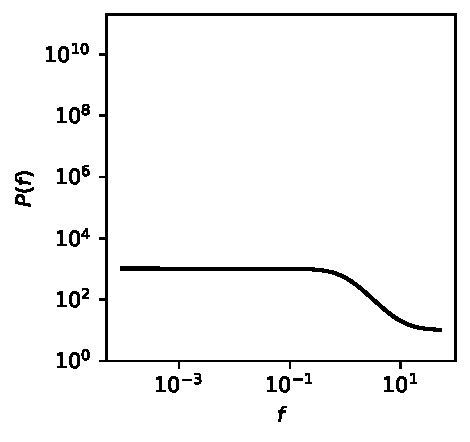
\includegraphics[width=\linewidth]
        {./images/0.1/small_condition_num/P_f.pdf}
    \caption{}
    \label{small condi num power spectrum CG}
\end{subfigure}%
\begin{subfigure}{0.33\textwidth}
    \centering
    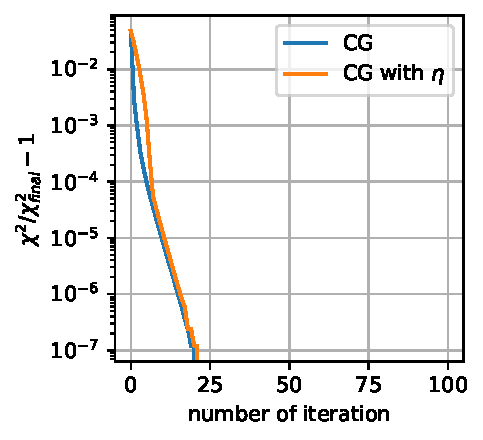
\includegraphics[width=\linewidth]
        {./images/0.1/small_condition_num/chi2_CG.pdf}
    \caption{}
    \label{small condi num chi2 CG}
\end{subfigure}%
\begin{subfigure}{0.33\textwidth}
    \centering
    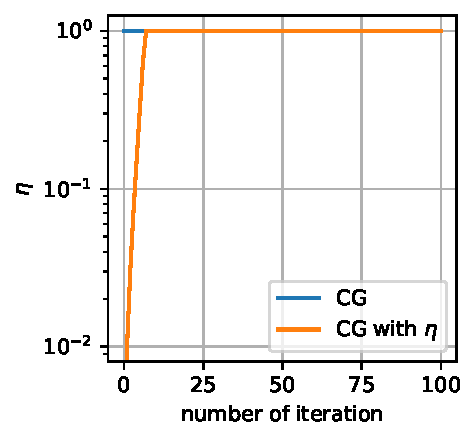
\includegraphics[width=\linewidth]
        {./images/0.1/small_condition_num/eta_CG.pdf}
    \caption{}
    \label{small condi num eta CG}
\end{subfigure}
\caption{The left graph shows the noise power spectrum
    Eq.(\ref{noise power spectrum}) with $f_{\text{apo}} \approx 0.99$ and
    $\kappa(N) = 10^2$. The center one shows the
    $\chi^2(\vbm)/\chi^2_{\text{final}} - 1$, with $\chi^2(\vbm)$ calculated
    based on Eq.(\ref{chi2 formula}).
    The right one shows the $\eta$ value for each iteration. For vanallia 
    conjugate gradient method $\eta$ always equal to $1$, so it's a horizontal
    line at $\eta=1$.
}
\label{small condi num CG}
\end{figure}

Notice that as we increase $\kappa(N)$, or equivalently decresing 
$f_{\text{apo}}$, the perturbative parameter $\eta$ starts showing its 
benefits, as showned in Figure(\ref{medium condi num CG}) and 
Figure(\ref{large condi num CG}).
It would outperforms vanilla conjugate gradient method, when 
$f_{\text{apo}} \approx 0$ and noise power spectrum becomes $1/f$ noise model,
which usually is the intrinsic noise of intruments\cite{1997PhRvD..56.4514T}.
\begin{figure}[htb]
\centering
\begin{subfigure}{0.33\textwidth}
    \centering
    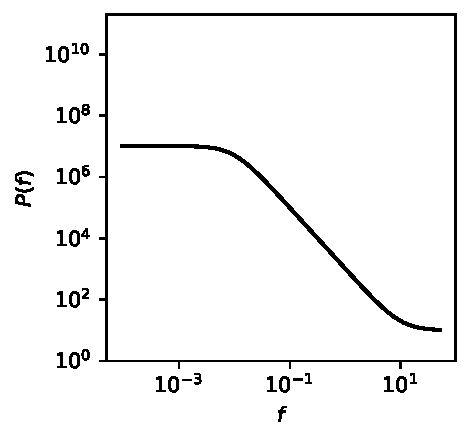
\includegraphics[width=\linewidth]
        {./images/0.1/medium_condition_num/P_f.pdf}
    \caption{}
    \label{medium condi num power spectrum CG}
\end{subfigure}%
\begin{subfigure}{0.33\textwidth}
    \centering
    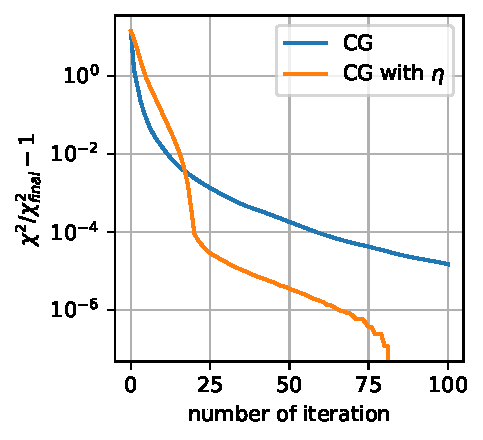
\includegraphics[width=\linewidth]
        {./images/0.1/medium_condition_num/chi2_CG.pdf}
    \caption{}
    \label{medium condi num chi2 CG}
\end{subfigure}%
\begin{subfigure}{0.33\textwidth}
    \centering
    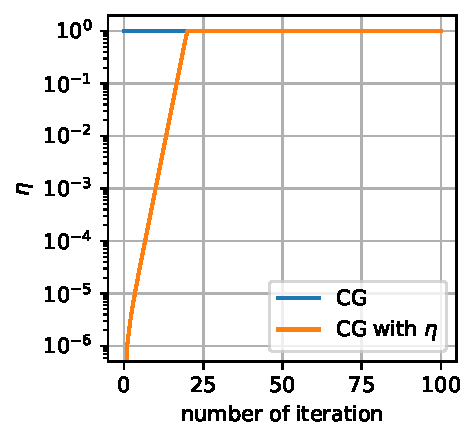
\includegraphics[width=\linewidth]
        {./images/0.1/medium_condition_num/eta_CG.pdf}
    \caption{}
    \label{medium condi num eta CG}
\end{subfigure}
\caption{The figure shows results for $f_{\text{apo}}\approx 9.8\times10^{-3}$ 
    and $\kappa(N) = 10^6$.
}
\label{medium condi num CG}
\end{figure}

\begin{figure}[htb]
\centering
\begin{subfigure}{0.33\textwidth}
    \centering
    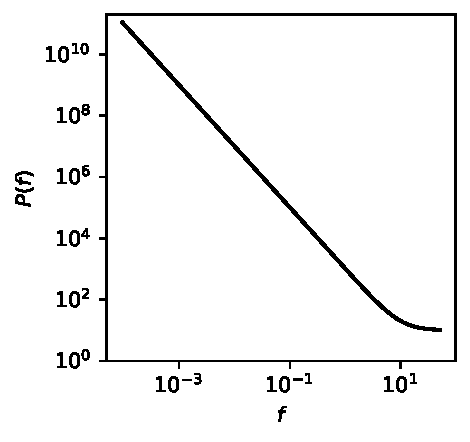
\includegraphics[width=\linewidth]
        {./images/0.1/large_condition_num/P_f.pdf}
    \caption{}
    \label{large condi num power spectrum CG}
\end{subfigure}%
\begin{subfigure}{0.33\textwidth}
    \centering
    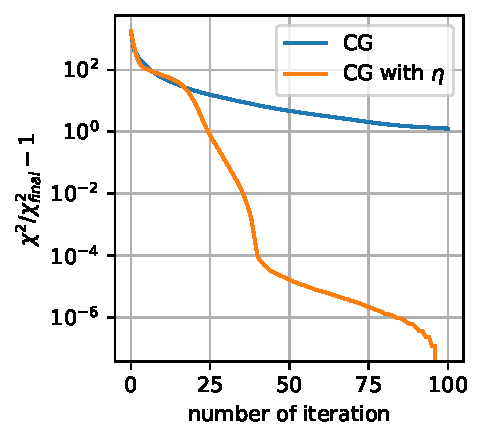
\includegraphics[width=\linewidth]
        {./images/0.1/large_condition_num/chi2_CG.pdf}
    \caption{}
    \label{large condi num chi2 CG}
\end{subfigure}%
\begin{subfigure}{0.33\textwidth}
    \centering
    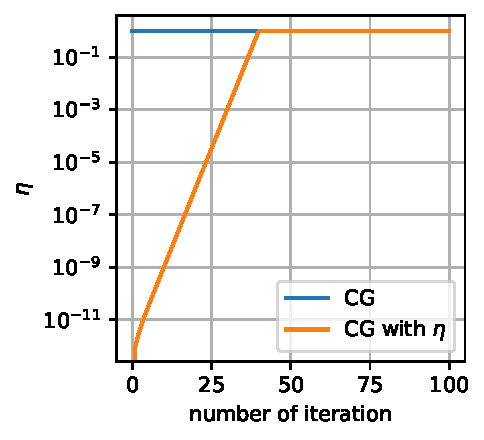
\includegraphics[width=\linewidth]
        {./images/0.1/large_condition_num/eta_CG.pdf}
    \caption{}
    \label{large condi num eta CG}
\end{subfigure}
\caption{The figure shows results for $f_{\text{apo}}\approx 9.8\times10^{-6}$ 
    and $\kappa(N) = 10^{12}$.
}
\label{large condi num CG}
\end{figure}

In conjugate gradient method with messenger cooling parameter $\lambda$, 
the number of cooling parameters we need is an extra free parameter.
After the number of $\lambda$ is determined, we construct a geometric series
with fixed initial and final value, which uses \texttt{logspace}
function in \texttt{numpy}.
Since I've showned in Eq.(\ref{lambda eta equiv}) that the messenger field
cooling parameter $\lambda$ is equivalent to $1/\eta$.
I would use $\eta$ for further analysis.

Now let's compare the performance difference between choosing $\eta$
parameters based on Eq.(\ref{etai rule})
and fixing number of $\eta$ parameters $n_{\eta}$ manully.
Here we choose the $\eta_i$ values using funtion
\texttt{numpy.logspace(start=$\ln(\eta_1)$, stop=0, num=$n_{\eta}$, base=$e$)}.
The results are showned in Figure(\ref{small condi num}),
(\ref{medium condi num}), and (\ref{large condi num}).

When $\kappa(N)$ is small, and Eq.(\ref{etai rule}) tells us that only a few
$\eta$ parameters are good enough, see Figure(\ref{small condi num chi2}).
If unfortunately we choose $n_{\eta}$ being large value, like $15$ or $30$,
then it will ends up converge slowly, because it need at least $15$ or $30$
iterations to reach $\eta=1$.

On the other hand if $\kappa(N)$ is very large and power spectrum is $1/f$
noise, we need more $\eta$ parameters.
If $n_{\eta}$ is too small, for example $n_{\eta}=5$ in
Figure(\ref{large condi num chi2}), which is better than vanilla conjugate
gradient method, but still far from optimal.


\begin{figure}[htb]
\centering
\begin{subfigure}{0.33\textwidth}
    \centering
    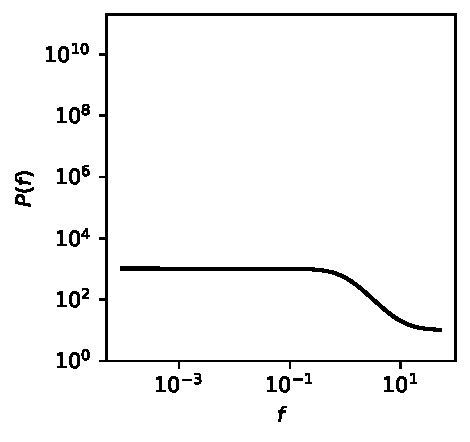
\includegraphics[width=\linewidth]
        {./images/0.1/small_condition_num/P_f.pdf}
    \caption{}
    \label{small condi num power spectrum}
\end{subfigure}%
\begin{subfigure}{0.33\textwidth}
    \centering
    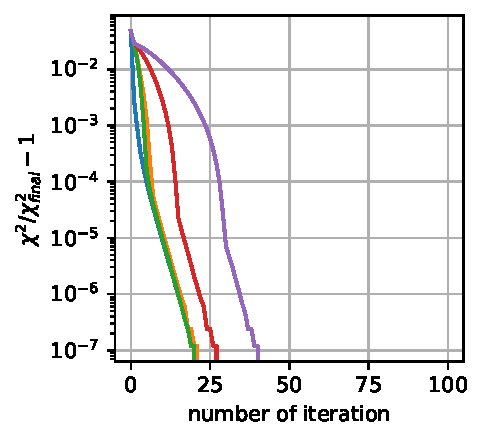
\includegraphics[width=\linewidth]
        {./images/0.1/small_condition_num/chi2.pdf}
    \caption{}
    \label{small condi num chi2}
\end{subfigure}%
\begin{subfigure}{0.33\textwidth}
    \centering
    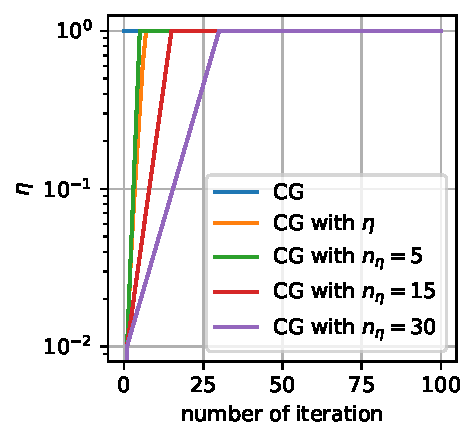
\includegraphics[width=\linewidth]
        {./images/0.1/small_condition_num/eta.pdf}
    \caption{}
    \label{small condi num eta}
\end{subfigure}
\caption{Same as Figure(\ref{small condi num CG}) with extra manully choosen 
    $n_{\eta}$ results.
}
\label{small condi num}
\end{figure}


\begin{figure}[htb]
\centering
\begin{subfigure}{0.33\textwidth}
    \centering
    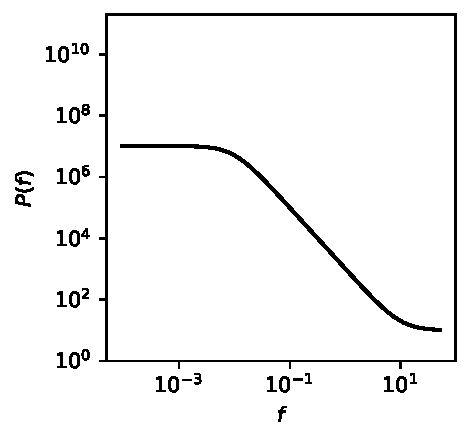
\includegraphics[width=\linewidth]
        {./images/0.1/medium_condition_num/P_f.pdf}
    \caption{}
    \label{medium condi num power spectrum}
\end{subfigure}%
\begin{subfigure}{0.33\textwidth}
    \centering
    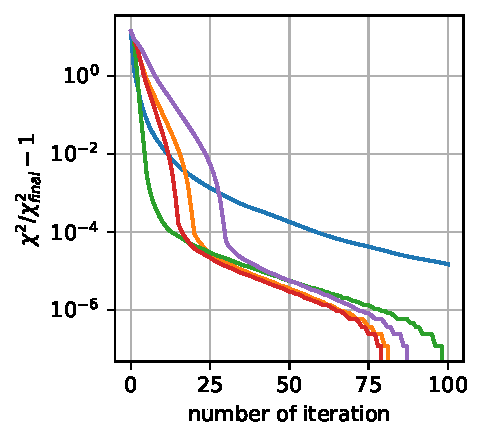
\includegraphics[width=\linewidth]
        {./images/0.1/medium_condition_num/chi2.pdf}
    \caption{}
    \label{medium condi num chi2}
\end{subfigure}%
\begin{subfigure}{0.33\textwidth}
    \centering
    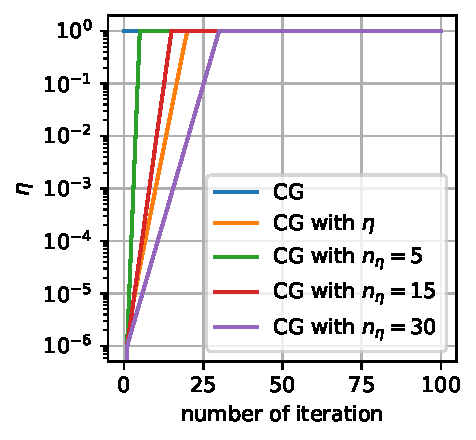
\includegraphics[width=\linewidth]
        {./images/0.1/medium_condition_num/eta.pdf}
    \caption{}
    \label{medium condi num eta}
\end{subfigure}
\caption{Same as Figure(\ref{medium condi num CG}) with extra manully choosen 
    $n_{\eta}$ results.
}
\label{medium condi num}
\end{figure}

\begin{figure}[htb]
\centering
\begin{subfigure}{0.33\textwidth}
    \centering
    \includegraphics[width=\linewidth]
        {./images/0.1/large_condition_num/p_f.pdf}
    \caption{}
    \label{large condi num power spectrum}
\end{subfigure}%
\begin{subfigure}{0.33\textwidth}
    \centering
    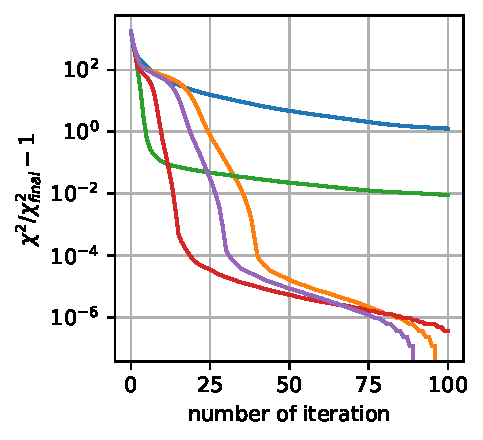
\includegraphics[width=\linewidth]
        {./images/0.1/large_condition_num/chi2.pdf}
    \caption{}
    \label{large condi num chi2}
\end{subfigure}%
\begin{subfigure}{0.33\textwidth}
    \centering
    \includegraphics[width=\linewidth]
        {./images/0.1/large_condition_num/eta.pdf}
    \caption{}
    \label{large condi num eta}
\end{subfigure}
\caption{Same as Figure(\ref{large condi num CG}) with extra manully choosen 
    $n_{\eta}$ results.
}
\label{large condi num}
\end{figure}

\section{Possible improvements}
As you may have noticed in Figure(\ref{medium condi num})
and Figure(\ref{large condi num}), the perturbative parameter based on
Eq.(\ref{etai rule}) is more than needed, especially for $1/f$ noise case.
From Figure(\ref{large condi num eta}) we know that Eq.(\ref{etai rule}) gives
us $n_{\eta}\approx40$, however based on $\chi^2$ result in 
Figure(\ref{large condi num chi2}), we notice that $n_{\eta}\approx30$ or 
even $n_{\eta} \approx 15$ is good enough.
Also, for the almost white noise case, we couls certainly choose $n_{\eta}=1$
such that $\eta_1=1$ which corresponds to vanallia conjugate gradient method,
based on $\chi^2$ result in Figure(\ref{small condi num chi2}).
However Eq.(\ref{etai rule}) gives us $n_{\eta} \approx 6$,
see Figure(\ref{small condi num eta}), eventhough it doesn't make final 
$\chi^2$ result much different at the end.

Is it possible to further improve the analysis, such that it produces
smaller $n_{\eta}$?
Let's examine how we get $\eta_i$ series.
Remember that we determine $\delta\eta$ value based on the upper bound of 
$-\delta\chi^2(\hatm(\eta), \eta)/\chi^2(\hatm(\eta), \eta)$, in
Eq.(\ref{eta upper bound}).
Here I rewrite it in a simplfied form
\begin{align}
-\frac{\delta\chi^2(\hatm(\eta), \eta)}{\chi^2(\hatm(\eta), \eta)}
= -\delta\eta
    \frac{\dv{\eta} \chi^2(\hatm(\eta), \eta)}
    {\chi^2(\hatm(\eta), \eta)}
= \delta\eta \frac{\hat{\vb{r}}_{\eta}^{\dagger} \inv{N}_{\eta} \Nbar 
    \inv{N}_{\eta} \hat{\vb{r}}_{\eta} }
    {\hat{\vb{r}}_{\eta}^{\dagger} \inv{N}_{\eta} \hat{\vb{r}}_{\eta} }
\leq  \frac{\delta \eta}{\eta + \frac{\tau}{\max(N_f) -\tau}}
\end{align}
with
$\vb{r}_{\eta} = \vbd - P\hatm(\eta) 
= \qty[ 1 - P\PPinv{\inv{N_{\eta}}}\Pdagger \inv{N_{\eta}}]\vbd
\equiv \mathcal{P}_{\eta} \vbd$.
We treated $\vb{r}_{\eta}$ as an arbitary 
vector in frequency domain, since we don't know how to calculate 
$\mathcal{P}_{\eta}$ for $\eta \neq 0$, and it's hard to 
analysize the projection matrix $\mathcal{P}_{\eta}$ in frequency space,
as it contains $\PPinv{\inv{N_{\eta}}}$.
Note that we have to determine all of $\eta$ value before calculation, 
because we don't want to keep time ordered data in system RAM,
so we need somehow analytically analysis $\mathcal{P}_{\eta}$, and its behavior
in frequency space.

Unless $\vb{r}_{\eta}$ almost only has large noise modes,
$\dv{\eta}\chi^2(\hatm(\eta),\eta)/\chi^2(\hatm(\eta),\eta)$
won't get close to the upper bound
$1/\qty(\eta + \frac{\tau}{\max(N_f) -\tau})$.
Based on the analysis in Section(\ref{intuitive interp}),
for small $\eta$ the estimated map $\hatm(\eta)$ does not only focusing on 
minimizing error $\vb{r}_{\eta}$ at low noise region.
So we would expect that there would be a fair amount of low noise modes
contribution in $\vb{r}_{\eta}$ especially for the first few $\eta$ values.
Which means if we could somehow know the frequncy distribution of 
$\vb{r}_{\eta}$, we could tighten the boundary of
$\dv{\eta}\chi^2(\hatm(\eta),\eta)/\chi^2(\hatm(\eta),\eta)$,
and get larger $\delta\eta$ value.
This should make $\eta$ goes to $1$ faster, and yields less $\eta$ parameters 
we need.

Also noting that the $\eta$ values determined from Eq.(\ref{etai rule})
\begin{align}
\eta_i =\min \qty\bigg{1,\; \frac{\tau}{\max(\Nbar_f)} \qty(2^i -1) } 
\tag{\ref{etai rule}}
\end{align}
are not dependent on any scaning information,
it only depends on noise power spectrum $P(f)$, or noise covariance matrix $N$.
Figure(\ref{large condi num 0.001}) and Figure(\ref{large condi num 10}) show
two examples with same parameters as in Figure(\ref{large condi num}) except 
scaning frequency $f_{\text{scan}}$, in Figure(\ref{large condi num 0.001}) it
scans very slow and in Figure(\ref{large condi num 10}) it's very fast.
In these two cases our $\eta$ values based on Eq.(\ref{etai rule}) are better
than manually selected values.
Based on these two results we know, the $\eta$ values should somehow depends
on scaning scheme.
Again that's because when we determine the upper bound of 
$\dv{\eta} \chi^2(\hatm(\eta), \eta)$ we treat
$\vb{r}_{\eta} = \vbd - P\hatm = \mathcal{P}_{\eta} \vbd$
as an arbitary vector, such that we lose all information related to scaning 
scheme in the pointing matrix $P$.


\begin{figure}[htb]
\centering
\begin{subfigure}{0.33\textwidth}
    \centering
    \includegraphics[width=\linewidth]
        {./images/0.001/large_condition_num/p_f.pdf}
    \caption{}
    \label{large condi num power spectrum 0.001}
\end{subfigure}%
\begin{subfigure}{0.33\textwidth}
    \centering
    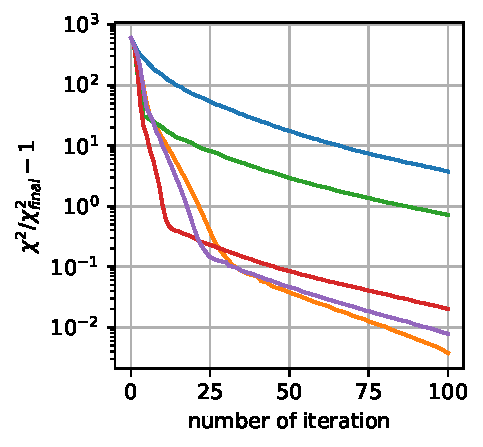
\includegraphics[width=\linewidth]
        {./images/0.001/large_condition_num/chi2.pdf}
    \caption{}
    \label{large condi num chi2 0.001}
\end{subfigure}%
\begin{subfigure}{0.33\textwidth}
    \centering
    \includegraphics[width=\linewidth]
        {./images/0.001/large_condition_num/eta.pdf}
    \caption{}
    \label{large condi num eta 0.001}
\end{subfigure}
\caption{In this case all frequencies are the same as
    Figure(\ref{large condi num}) except $f_{\text{scan}} = 0.001$.
}
\label{large condi num 0.001}
\end{figure}

\begin{figure}[htb]
\centering
\begin{subfigure}{0.33\textwidth}
    \centering
    \includegraphics[width=\linewidth]
        {./images/10/large_condition_num/p_f.pdf}
    \caption{}
    \label{large condi num power spectrum 10}
\end{subfigure}%
\begin{subfigure}{0.33\textwidth}
    \centering
    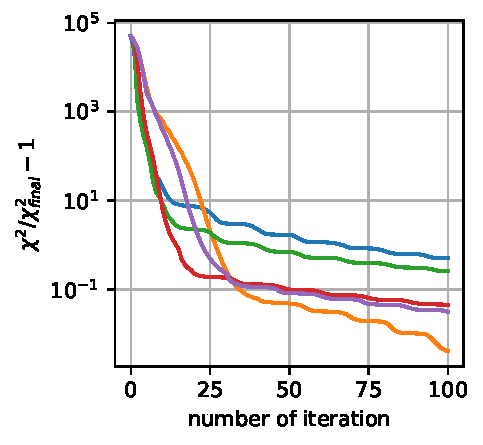
\includegraphics[width=\linewidth]
        {./images/10/large_condition_num/chi2.pdf}
    \caption{}
    \label{large condi num chi2 10}
\end{subfigure}%
\begin{subfigure}{0.33\textwidth}
    \centering
    \includegraphics[width=\linewidth]
        {./images/10/large_condition_num/eta.pdf}
    \caption{}
    \label{large condi num eta 10}
\end{subfigure}
\caption{In this case all frequencies are the same as
    Figure(\ref{large condi num}) except $f_{\text{scan}} = 10$.
}
\label{large condi num 10}
\end{figure}



\section{Conclusion}
Here we discussed a method to solve map making equation
Eq.(\ref{map making equation})
\begin{align}
\hatm = \PPinv{N} \Pdagger \inv{N} \vbd \tag{\ref{map making equation}}
\end{align}
by seperate noise covariance matrix $N$ into two parts, white noise part
$\tau I$ and the remaining noise $\Nbar$.
Then we could think $\Nbar$ as a perturbation added to white noise, 
by introducing a parameter $\eta$, as $\eta$ change from $0$ to $1$,
we gradually add this non white noise in to system.

The $\eta$ values can be predetermined analytically.
This property is very important, because we don't want to keep entire time
ordered data in system RAM.
If these $\eta$ values can be determined before calculation, then we only need
to keep several map sized object, which is much smaller than timer ordered 
data.
Also we showed that this method has same computational cost as vanilla
conjugate gradient method but performs better when the condition number of 
noise covariance matrix $\kappa(N)$ is large, especially in $1/f$ noise case.
The only extra free parameter added is to determine whether the error at
current step $\vb{r}(\eta_i) = \qty||\vbb(\eta_i) - A(\eta_i) \vbm||$ is small
enough such that we change advance to next value $\eta_{i+1}$.

The perturbative parameter $\eta$ get from Eq.(\ref{etai rule}) are not
prefect. Since it only takes in to account the noise information in $N$,
but ignored all scaning information contained in pointing matrix $P$, because
we are unable to analysis the pattern of
$\vb{r}_{\eta} = \vbd - P\hatm(\eta) = \mathcal{P}_{\eta} \vbd$ in frequency
space.

The analysis of $\eta$ value also explains why cooling parameters
$\lambda=1/\eta$ in messenger field are choosen to be geometric series or
\texttt{logspace} \cite{Huffenberger_2018}.

All of the calculation are using simple preconditioner $\Pdagger P$, but 
the entire analysis is independent of preconditioner.
So if using better preconditioners, it would also have improvements.





\medskip

\bibliographystyle{plain}
\bibliography{references.bib}




\end{document}


